%! TEX root = ../ag-19-20.tex

\chapter{Conice și cuadrice}

\section{Conice}

Conicele sînt curbe plane, date de ecuații pătratice. Ele sînt reprezentate
în figura \ref{figure:conice}, împreună cu ecuațiile canonice.

\begin{figure}[!htbp]
  \centering
  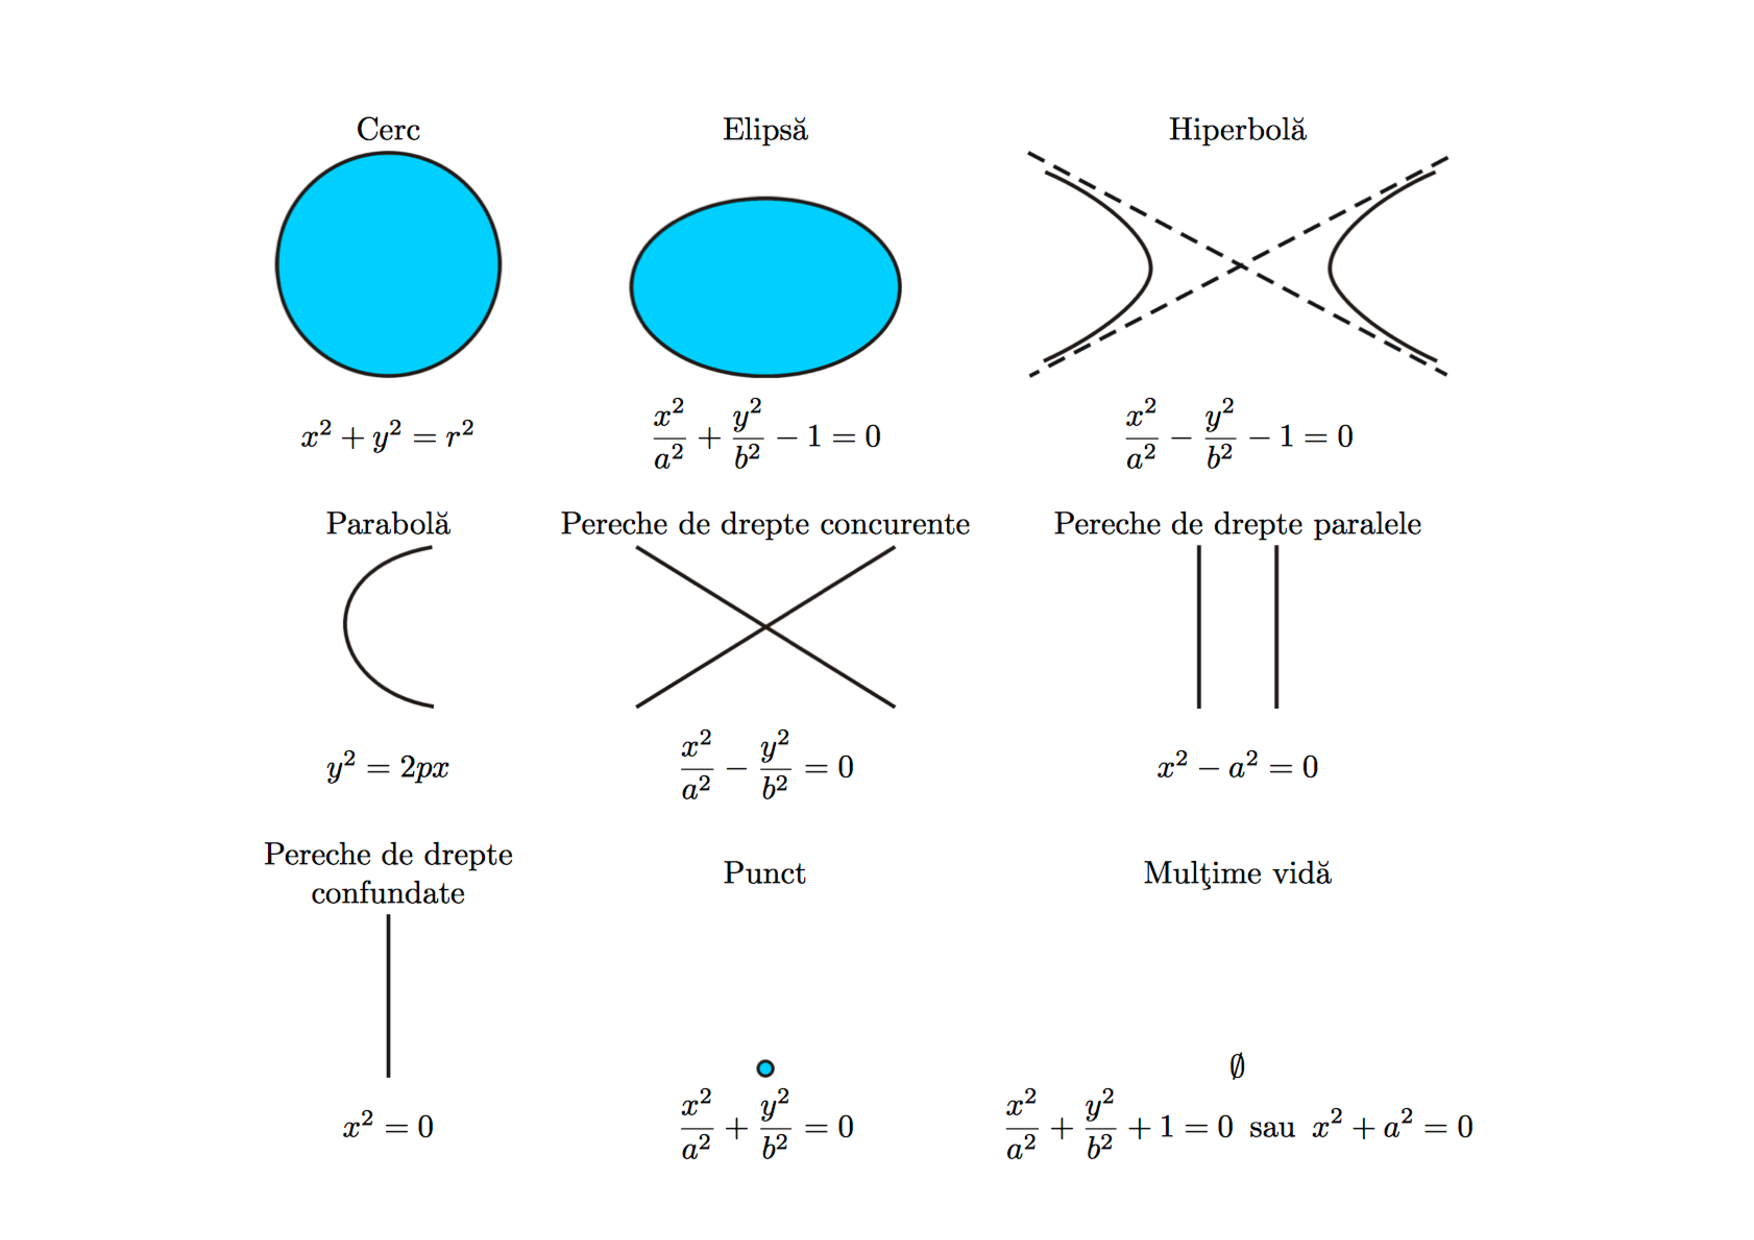
\includegraphics[scale = 0.5]{figs/conice}
  \caption{Conice și ecuațiile lor}
  \label{figure:conice}
\end{figure}

Scopul pe care ni-l propunem în această secțiune este să aducem o ecuație
a unei conice la forma canonică și să o reprezentăm grafic.

Vom prezenta algoritmul direct pe un exemplu. Metoda aplicată se
numește \emph{metoda rototranslației}, deoarece va folosi o operație
de rotație și una de translație a conicei.

Fie, de exemplu, conica:
\[
  g(x, y) = 3x^2 - 4xy - 2x + 4y - 3 = 0.
\]

Mai întîi, se scrie \emph{forma pătratică asociată}, adică alegem din conică
termenii de grad total 2:
\[
  q(x, y) = 3x^2 - 4xy.
\]

Apoi, scriem \emph{matricea asociată lui $q$}, care este:
\[
  A = \begin{pmatrix}
    3 & -2 \\
    -2 & 0
  \end{pmatrix}
\]

Această matrice se obține punînd coeficienții termenilor pătratici, în ordine
lexicografică. Dacă $ C(t) $ notează coeficientul termenului $ t $, atunci
matricea este, în forma generică:
\[
  A = \begin{pmatrix}
    C(x^2) & C(xy) \\
    C(yx) & C(y^2)
  \end{pmatrix},
\]
cu convenția că $ C(xy) = C(yx) $, deci în matrice vom avea jumătate din
coeficientul din forma pătratică.

Pentru această matrice, scriem ecuația caracteristică:
\[
  P_A(X) = \det(A - XI_2) = X^2 - 3X - 4 = (X + 1)(X - 4).
\]

Rezultă că valorile proprii sînt $ \sigma(A) = \{-1, 4 \} $.

În acest punct, putem face o observație de anticipație. Se numește
\emph{invariantul $ \delta $} al conicei produsul valorilor proprii.
Avem cazurile:
\begin{itemize}
\item $ \delta = \lambda_1 \cdot \lambda_2 > 0 \Rightarrow $ conica este elipsă;
\item $ \delta = \lambda_1 \cdot \lambda_2 < 0 \Rightarrow $ conica este hiperbolă;
\item $ \delta = \lambda_1 \cdot \lambda_2 = 0 \Rightarrow $ conica este parabolă.
\end{itemize}

În cazul nostru, vom obține o hiperbolă.

Mai departe, se calculează vectorii proprii și obținem:
\[
  V(\lambda_1) = \dr{Sp} \{(1, 2) \}, \quad V(\lambda_2) = \dr{Sp} \{(2, -1) \}.
\]

Vectorii din bazele subspațiilor proprii trebuie \emph{ortonormați} (de exemplu,
folosind procedura Gram-Schmidt). Observăm că ei sînt deja ortogonali, deci
mai trebuie doar să-i normăm:
\[
  ||(1, 2)|| = ||(2, -1)|| = \sqrt{5},
\]
deci obținem \emph{versorii proprii:}
\[
  e_1 = \Big(\frac{1}{\sqrt{5}}, \frac{2}{\sqrt{5}} \Big), \quad %
  e_2 = \Big(\frac{2}{\sqrt{5}}, \frac{-1}{\sqrt{5}} \Big)
\]

Acești versori vor alcătui coloanele \emph{matricei de rotație}:
\[
  R = \begin{pmatrix}
    \dfrac{1}{\sqrt{5}} & \dfrac{2}{\sqrt{5}} \\
                       & \\
    \dfrac{2}{\sqrt{5}} & \dfrac{-1}{\sqrt{5}}
  \end{pmatrix}
\]

În general, o matrice de rotație de unghi $ \theta $ (în sens trigonometric)
are forma:
\[
  R_\theta = \begin{pmatrix}
    \cos \theta & -\sin \theta \\
    \sin \theta & \cos \theta
  \end{pmatrix}
\]
și $ \det R_\theta = 1 $.

În cazul nostru, $ \det R = -1 $, deci putem schimba între ele coloanele
și obținem o matrice de rotație (echivalent, putem schimba orientarea unuia
dintre versori, de exemplu, $ e_1 \longrightarrow -e_1 $).

Apoi aplicăm rotația, adică, dacă $ (x, y) $ sînt vechile coordonate,
coordonatele din sistemul rotit $ (x', y') $ se obțin din ecuația:
\[
  \begin{pmatrix}
    x \\ y
  \end{pmatrix} = R \cdot \begin{pmatrix} x_1 \\ y_1 \end{pmatrix}
\]

Cu alte cuvinte, avem sistemul:
\[
  \begin{cases}
    x &= \dfrac{-1}{\sqrt{5}} x_1 + \dfrac{2}{\sqrt{5}} y_1 \\
      & \\
    y &= \dfrac{-2}{\sqrt{5}} x_1 + \dfrac{-1}{\sqrt{5}} y_1
  \end{cases}.
\]

Aceste coordonate se înlocuiesc în ecuația inițială a conicei și obținem
\emph{conica rotită}:
\[
  -x_1^2 + 4y_1^2 - \frac{6}{\sqrt{5}} x_1 - \frac{8}{\sqrt{5}} y_1 - 3 = 0.
\]

Prelucrăm algebric, completînd pătratele, și obținem:
\[
  -\Big( x_1 + \frac{3}{\sqrt{5}} \Big)^2 + 4 \Big(y_1 - \frac{1}{\sqrt{5}} \Big)^2 = 2.
\]

Facem acum \emph{translația}:
\[
  \begin{cases}
    X &= x_1 + \dfrac{3}{\sqrt{5}} \\
      & \\
    Y &= y_1 - \dfrac{1}{\sqrt{5}}
  \end{cases}
\]
și obținem:
\[
  -X^2 + 4Y^2 = 2 \Leftrightarrow %
  -\Big( \frac{X}{\sqrt{2}} \Big)^2 + \Big( \frac{Y}{1/2} \Big)^2 = 1,
\]
deci ecuația unei hiperbole.

Pentru reprezentarea grafică, trebuie să ținem cont de operațiile efectuate:
\begin{itemize}
\item rotația de unghi $ \theta $, cu proprietatea că $ \cos \theta = -\dfrac{1}{\sqrt{5}} $,
  deci $ \theta \simeq \dfrac{2\pi}{3} $;
\item translația centrului cu $ \dfrac{3}{\sqrt{5}} $ pe axa $ OX $ și
  $ -\dfrac{1}{\sqrt{5}} $ pe axa $ OY $.
\end{itemize}

Mai putem determina și \emph{centrul conicei}, din sistemul:
\[
  \begin{cases}
    \dfrac{\partial g}{\partial x} &= 0 \\
    & \\    
    \dfrac{\partial g}{\partial y} &= 0
  \end{cases}
\]

Soluția sistemului este centrul conicei, de coordonate $ C(1, 1) $.

Reprezentarea grafică (folosind \href{https://www.geogebra.org/}{GeoGebra}) este
redată în figura \ref{fig:hiperbola-geog}.

\begin{figure}[!htbp]
  \centering
  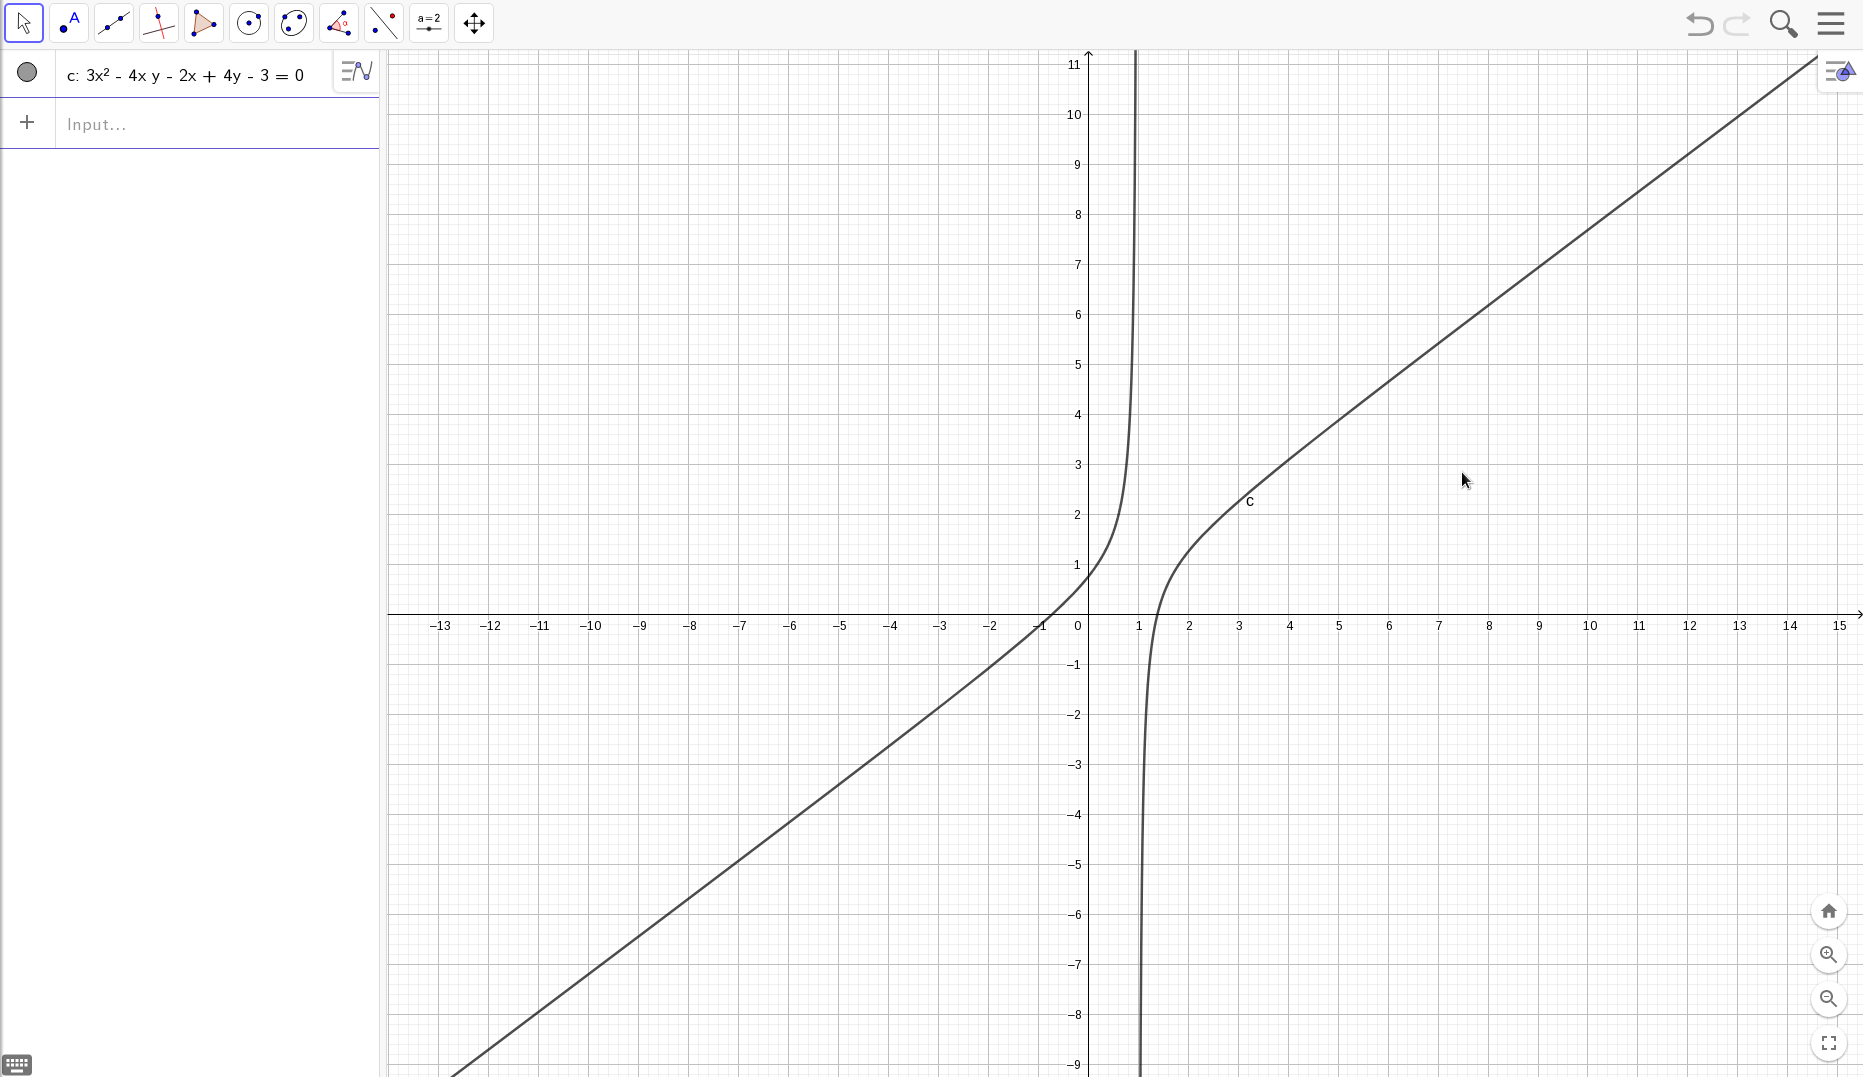
\includegraphics[scale = 0.3]{figs/hiperbola-geogebra.png}
  \caption{Hiperbola $3x^2 - 4xy - 2x + 4y - 3 = 0$}
  \label{fig:hiperbola-geog}
\end{figure}

\textbf{OBSERVAȚIE:} O metodă alternativă este să pornim cu calculul centrului.
Atunci, primul pas al transformării este \emph{translația în centru}.
Astfel, în exemplul de mai sus, calculăm mai întîi centrul $ C(1, 1) $,
iar apoi facem substituția în forma $ g(x, y) $, adică $ x \mapsto (x + 1) $
și $ y \mapsto (y + 1) $, deci:
\begin{align*}
    g(x, y) &= 3(x + 1)^2 - 4(x + 1)(y + 1) - 2(x + 1) + 4(y + 1) - 3 \\
            &= 3x^2 - 4xy,
\end{align*}
care coincide cu forma pătratică considerată în metoda inițială.

Din acest punct, putem continua cu rotația ca mai sus.

%%%%%%%%%%%%%%%%%%%%%%%%%%%%%%%%%%%%%%%%%%%%%%%%%%%%%%%%%%%%%%%%%%%%%% 

\section{Cuadrice}

Cuadricele sînt suprafețe care pot fi obținute prin rotirea unei conice în jurul
unei axe. Astfel, din elipsă, de exemplu, obținem elipsoizi, din parabolă,
paraboloizi, iar din hiperbolă, hiperboloizi.

Formele, împreună cu ecuațiile canonice, pot fi consultate, de exemplu,
\href{https://en.wikipedia.org/wiki/Quadric#Euclidean_space}{aici}.

Procedura de a aduce o cuadrică la forma canonică funcționează ca în cazul
conicelor.

Mai jos un exemplu rezolvat.

\[
  x^2 + 3y^2 + 4yz - 6x + 8y + 8 = 0.
\]

Considerăm forma pătratică asociată:
\[
  g = x^2 + 3y^2 + 4yz,
\]
care are matricea simetrică.
\[
  A = \begin{pmatrix}
    1 & 0 & 0 \\
    0 & 3 & 2 \\
    0 & 2 & 0
  \end{pmatrix}
\]
Ecuația caracteristică rezultă: $(1 - \lambda)(\lambda^2 - 3\lambda - 4) = 0$,
deci $\lambda_1 = 1, \lambda_2 = -1, \lambda_3 = 4$.

Găsim subspațiile invariante:
\begin{align*}
  V(\lambda_1) &= \Bigg\{ (x, y, z) \in \RR^3 \mid %
                 \begin{pmatrix}
                   0 & 0 & 0 \\
                   0 & 2 & 2 \\
                   0 & 2 & -1
                 \end{pmatrix} \cdot
                           \begin{pmatrix}
                             x \\ y \\ z
                           \end{pmatrix}  =
  \begin{pmatrix}
    0 \\ 0 \\ 0
  \end{pmatrix} \Bigg\} \\
               &= \{ (x, 0, 0) \mid x \in \RR \}
\end{align*}

Similar:
\begin{align*}
  V(\lambda_2) &= \{ (0, y, -2y) \mid y \in \RR \} \\
  V(\lambda_3) &= \{ (0, 2z, z) \mid z \in \RR \}.
\end{align*}

Alegem vectori proprii ortonormați particularizînd elemente din
subspațiile invariante.
De exemplu:
\[
  e_1 = (1, 0, 0), \quad e_2 = \frac{1}{\sqrt{5}} (0, 1, -2), %
  \quad e_3 = \frac{1}{\sqrt{5}}(0, 2, 1).
\]
Matricea $R$ cu acești vectori pe coloane are proprietatea $\det R = 1$, deci
este o matrice de rotație. O aplicăm și găsim schimbarea de coordonate:
\[
  \begin{cases}
    x &= x' \\
    y &= \dfrac{1}{\sqrt{5}} (y' + 2z') \\
      & \\
    z &= \dfrac{1}{\sqrt{5}} (-2y' + z')
  \end{cases}
\]

Ecuația cuadricei devine:
\[
  x^{\prime 2} - y^{\prime 2} + 4 z^{\prime 2} - 6x^\prime + %
  \frac{8}{\sqrt{5}} y^\prime + \frac{16}{\sqrt{5}} z^\prime + 8 = 0.
\]

Formăm pătrate și obținem:
\[
  (x' - 3)^2 - \big( y' - \frac{4}{\sqrt{5}} \big)^2 + %
  4 \big(z' + \frac{2}{\sqrt{5}} \big)^2 - 1 = 0.
\]

Efectuăm translația corespunzătoare noilor coordonate și obținem:
\[
  X^2 - Y^2 + 4Z^2 - 1 = 0 \Leftrightarrow X^2 - Y^2 + \frac{Z^2}{\frac{1}{4}} - 1 = 0,
\]
adică un hiperboloid cu o pînză.

%%%%%%%%%%%%%%%%%%%%%%%%%%%%%%%%%%%%%%%%%%%%%%%%%%%%%%%%%%%%%%%%%%%%%%

\section{Exerciții propuse}

\indent\indent 1. Aduceți următoarele conice la forma canonică și reprezentați-le:
\begin{enumerate}[(a)]
\item $ 4xy - 3y^2 + 4x - 14y - 7 = 0 $ (hiperbolă);
\item $ 9x^2 - 6xy + y^2 + 20x = 0 $ (parabolă);
\item $ x^2 - 2xy + y^2 - 5x + y - 2 = 0 $ (parabolă);
\item $ 5x^2 + 8xy + 5y^2 - 18x - 18y + 9 = 0 $ (elipsă);
\item $ x^2 - 4xy + 4y^2 - 6x + 2y + 1 = 0 $ (parabolă)
\end{enumerate}

\vspace{1cm}

2. Aceeași cerință pentru cuadrica:
\[
  x^2 - y^2 + z^2 - 2xy - 2yz - 2zx - 5x - 1 = 0
\]
(hiperboloid cu o pînză).


%%% Local Variables:
%%% mode: latex
%%% TeX-master: "../ag-19-20"
%%% End:
